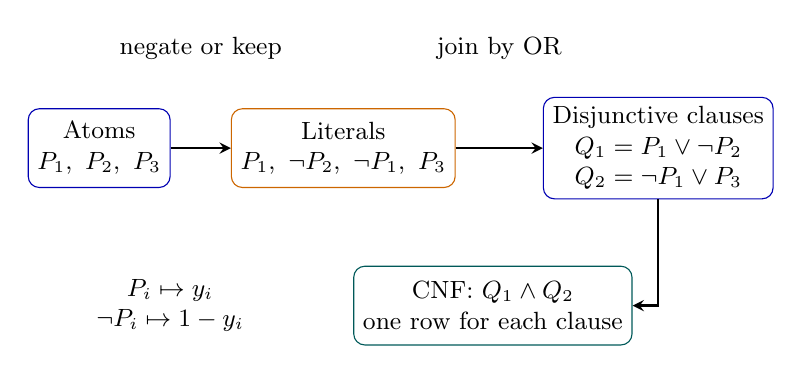
\begin{tikzpicture}[>=stealth,box/.style={draw,rounded corners,align=center,minimum height=1cm,font=\small}]
\node[box,draw=blue!70!black] (a) at (0,0) {Atoms\\$P_1,\ P_2,\ P_3$};
\node[box,draw=orange!80!black] (l) at (3.1,0) {Literals\\$P_1,\ \neg P_2,\ \neg P_1,\ P_3$};
\node[box,draw=blue!70!black] (q) at (7.1,0) {Disjunctive clauses\\$Q_1=P_1\lor\neg P_2$\\$Q_2=\neg P_1\lor P_3$};
\draw[->,thick] (a)--node[above=10mm,font=\small]{negate or keep}(l);
\draw[->,thick] (l)--node[above=10mm,font=\small]{join by OR}(q);
\node[box,draw=teal!70!black] (c) at (5,-2) {CNF: $Q_1\land Q_2$\\one row for each clause};
\draw[->,thick] (q.south)--(q.south|-c.east)--(c.east);
\node[font=\small,align=center] at (0.9,-2) {$P_i\mapsto y_i$\\$\neg P_i\mapsto1-y_i$};
\end{tikzpicture}
